\chapter{Analisi dei componenti}
    Nel presente capitolo viene presentata l'architettura in termini di componenti (CMP) interni al sistema definiti sulla base dei requisiti analizzati in precedenza.

\section{Definizione dei componenti}
    Definiamo di seguito i componenti del sistema con le relative funzionalità.
    
    \subsection{\texttt{CMP1}: Gestione grafici}
        \subsubsection{Descrizione} 
            Il componente si occupa della funzionalità di generare per ogni attributo un grafico storico. Tale grafico raffigura l'andamento del relativo attributo in un dato arco di tempo.
        \subsubsection{Interfaccia richiesta - Selezione attributo:}
            Viene richiesta al \texttt{CMP} ``Gestione Attributi'' la selezione dell'attributo per il quale è necessario generare un grafico.
        \subsubsection{Interfaccia richiesta - Attributi:}
            Nella seguente interfaccia vengono richiesti al \texttt{CMP} ``Gestione Database'' i dati riguardanti l'attributo di interesse.
        \subsubsection{Interfaccia fornita - Grafico:}
            Il componente fornisce dunque il grafico raffigurante l'andamento nel tempo dell'attributo fornito.
    
    \subsection{\texttt{CMP2}: Gestione lingua}
        \subsubsection{Descrizione} 
            Il componente si occupa della funzionalità di generare in base alla lingua selezionata il testo presente nella pagina basandosi sui testi presenti all'interno di file JSON appositi.
        \subsubsection{Interfaccia richiesta - Selezione lingua:}
            Viene richiesta la selezione da parte dell'utente della lingua di preferenza.
            In caso di default la lingua selezionata sarà l'italiano.
        \subsubsection{Interfaccia fornita - Testo:}
            Il componente fornisce il testo necessario tradotto in base alla lingua selezionata in precedenza.

    \subsection{\texttt{CMP3}: Gestione mappa e tabella}
        \subsubsection{Descrizione}
            Il componente si occupa di fornire all'utente una rappresentazione dettagliata della città e delle suoi zone geografiche. Attraverso il seguente componente è inoltre possibile selezionare una delle zone geografiche per la quali si vuole ricevere maggiori informazioni. 
        \subsubsection{Interfaccia richiesta - Selezione zona:}
            Attraverso la seguente interfaccia il componente riceve dall'utente la zona geografica sulla quale vuole ricevere maggiori informazioni. Nel caso in cui non vi fosse una zona selezionata verrà utilizzata quella di default, ovvero l'intero comune.
        \subsubsection{Interfaccia richiesta - Testo:}
            Il testo comprende la traduzione dei dati forniti e dei nomi presenti nelle varie aree geografiche.
        \subsubsection{Interfaccia richiesta - Mappa di trento:}
            Fa una richiesta a \texttt{OpenStreetMap} per avere la mappa del comune.
        \subsubsection{Interfaccia fornita - Immagine:}
            Rappresentazione grafica tramite mappa della città o dell'area geografica selezionata.
        \subsubsection{Interfaccia fornita - Zona selezionata:}
            Indica agli altri componenti la zona selezionata sulla quale andranno effettuate, nel caso in cui si possedessero le autorizzazioni necessarie, le seguenti operazioni.
    
    \subsection{\texttt{CMP4}: Gestione attributi}
        \subsubsection{Descrizione}
            Il componente si occupa di fornire all'utente tutte le informazioni necessarie riguardo le zone geografiche o i servizi presenti all'interno di esse. Il seguente componente è dunque in grado di generare diverse rappresentazioni degli attributi in base alle autorizzazioni, alla zona o al servizio selezionato che arrivano in ingresso alle varie interfacce richieste.
        \subsubsection{Interfaccia richiesta - Testo:}
            Il testo comprende la traduzione dei vari attributi, servizi e delle categorie di attributi presenti all'interno delle varie rappresentazioni degli attributi.
        \subsubsection{Interfaccia richiesta - Zona selezionata:}
            Indica la zona per la quale bisogna visualizzare gli attributi principali. Nel caso in cui non vi fosse una zona selezionata verrà utilizzata quella di default, ovvero l'intero comune.
        \subsubsection{Interfaccia richiesta - Servizio selezionato:}
            Indica l'attributo per il quale bisogna visualizzare la lista dei servizi che svolgono un ruolo attivo, all'interno della zona selezionata, all'interno dell'ambito di tale attributo. Nel caso in cui non vi fosse un'attributo selezionato verrà utilizzata quella di default, ovvero nessun attributo.
        \subsubsection{Interfaccia richiesta - Autorizzazione:}
            \texttt{Bit} che segnala se l'utente ha il permesso necessario per compiere o meno un'azione.
        \subsubsection{Interfaccia richiesta - Attributi:}
            Nella seguente interfaccia vengono richiesti al \texttt{CMP} ``Gestione Database'' gli attributi di  interesse.
        \subsubsection{Interfaccia fornita - Selezione attributo:}
            Fornisce al \texttt{CMP} ``Gestione Grafici'' gli attributi per i quali è necessario fornire la rappresentazione di un grafico per uno studio ulteriore dell'andamento.
        \subsubsection{Interfaccia fornita - Valore attributi:}
            L'interfaccia fornisce una rappresentazione degli attributi presenti in base ai dati forniti all'interno delle interfacce richieste.

    \subsection{\texttt{CMP5}: Gestione database}
        \subsubsection{Descrizione} 
            Il componente si occupa di fornire la raccolta dei dati più importanti. Salva nel database tutti i dati relativi alle categorie e agli attributi stessi, tiene inoltre traccia dei voti e integra ciò con i voti presenti all'interno dei sondaggi valutati positivamente.
        \subsubsection{Interfaccia richiesta - Dati database:}
            Raccolta di tutti i dati presenti all'interno del database, questi dati riguardano gli attributi per il \texttt{CMP} ``Gestione Attributi'' e i voti per i vari \texttt{CMP} correlati.
        \subsubsection{Interfaccia richiesta - Dati strutture modificati:}
            Raccolta dei dati appartenenti ad una struttura che ha appena subito una modifica.
        \subsubsection{Interfaccia richiesta - Cancellazione sondaggio:}
            Codice identificativo che permette la rimozione di un sondaggio e di tutti i voti collegati al corrispettivo sondaggio dal database.
        \subsubsection{Interfaccia richiesta - Sondaggi approvati:}
            Codice identificativo che permette l'aggiunta di un sondaggio all'interno della lista di sondaggi accettati e l'aggiunta di tutti i voti collegati al corrispettivo sondaggio.
        \subsubsection{Interfaccia fornita - Attributi:}
            Il componente fornisce l'insieme degli attributi presenti all'interno del database che verranno filtrati nei successivi \texttt{CMP}.
        \subsubsection{Interfaccia fornita - Modifiche databse:}
            Raccolta di tutti i dati che sono stati modificati e che vanno dunque sostituiti all'interno della base di dati.
    
    \subsection{\texttt{CMP6}: Gestione dati strutture}
        \subsubsection{Descrizione}
            Il componente si occupa di permettere agli utenti che ne hanno l'autorizzazione di poter gestire i dati sui quali possono esercitare il controllo.
        \subsubsection{Interfaccia richiesta - Autorizzazione:}
            \texttt{Bit} che segnala se l'utente ha il permesso necessario per compiere o meno un'azione.
        \subsubsection{Interfaccia richiesta - Modifica dei dati:}
            Dati appartenenti ad una struttura i quali, in seguito, verranno inviati al database per poter essere modificati.
        \subsubsection{Interfaccia fornita - Dati strutture modificati:}
            Insieme dei dati appartenenti alla struttura che ha appena subito una modifica da un'utente autorizzato a compiere tale operazione.

    \subsection{\texttt{CMP7}: Gestione invio richieste}
        \subsubsection{Descrizione}
            Il componente si occupa di inviare le richieste, fornite da utenti con le corrispettive autorizzazioni, al \texttt{CMP} ``Gestione invio risposte'' e di gestire la corrispettiva risposta. Le richieste permetteranno di mettere in contatto diretto le circoscrizioni e il comune permettendo una comunicazione più efficiente.
        \subsubsection{Interfaccia richiesta - Testo richiesta:}
            Rappresenta il testo completo della richiesta fornito dalla circoscrizione.
        \subsubsection{Interfaccia richiesta - Risposte:}
            Racchiude il testo completo della risposta fornito dal comune e il codice identificativo della richiesta alla quale il messaggio sta rispondendo.
        \subsubsection{Interfaccia richiesta - Autorizzazione:}
            \texttt{Bit} che segnala se l'utente ha il permesso necessario per compiere o meno un'azione.
        \subsubsection{Interfaccia fornita -T esto risposte:}
            Racchiude il testo completo della richiesta fornito dalla circoscrizione con in coda il testo completo della risposta contrassegnato dall'utente che ha risposto.
        \subsubsection{Interfaccia fornita - Richieste:}
            Rappresenta il testo completo della richiesta, il codice identificativo della richiesta, il codice identificativo della circoscrizione ed il codice identificativo dell'utente che ha inviato la richiesta.

    \subsection{\texttt{CMP8}: Gestione invio risposte}
        \subsubsection{Descrizione}
            Il componente si occupa di fornire le risposte per le richieste inviate dal \texttt{CMP} ``Gestione invio risposte''. Le risposte permetteranno di semplificare la comunicazione diretta tra le circoscrizioni ed il comune stesso basandosi su di un servizio più efficiente.
        \subsubsection{Interfaccia richiesta - Richieste:}
            Rappresenta il testo completo della richiesta, il codice identificativo della richiesta, il codice identificativo della circoscrizione ed il codice identificativo dell'utente che ha inviato la richiesta.
        \subsubsection{Interfaccia richiesta - Testo risposta:}
            Rappresenta il testo completo della risposta fornito dal comune.
        \subsubsection{Interfaccia richiesta - Autorizzazione:}
            \texttt{Bit} che segnala se l'utente ha il permesso necessario per compiere o meno un'azione.
        \subsubsection{Interfaccia fornita - Risposte:}
            Racchiude il testo completo della risposta fornito dal comune e il codice identificativo della richiesta alla quale il messaggio sta rispondendo.
        \subsubsection{Interfaccia fornita - Testo richieste:}
            Rappresenta il testo completo della richiesta, il nome della circoscrizione ed il nome dell'utente che ha inviato la richiesta.

    \subsection{\texttt{CMP9}: Gestione voti}
        \subsubsection{Descrizione}
            Il componente si occupa di permettere ai sondaggisti di aggiungere o eliminare i voti. Nel momento di aggiunta del voto oltre al valore del voto devono anche essere inserite una serie di informazioni base del cittadino votante.
        \subsubsection{Interfaccia richiesta - Autorizzazione:}
            \texttt{Bit} che segnala se l'utente ha il permesso necessario per compiere o meno un'azione.
        \subsubsection{Interfaccia richiesta - Informazioni cittadino:}
            Insieme dei dati riguardanti l'età e il quartiere di provenienza del cittadino votante.
        \subsubsection{Interfaccia richiesta - Valore voto:}
            Valore numerico che rappresenta il grado di soddisfazione del cittadino.
        \subsubsection{Interfaccia fornita - Voti:}
            Insieme di informazioni che racchiude l'insieme dei voti e delle informazioni generiche riguardanti i cittadini che hanno votato.

    \subsection{\texttt{CMP10}: Gestione sondaggi}
        \subsubsection{Descrizione}
            Il componente si occupa di permettere ai sondaggisti di modificare, aggiungere, completare o eliminare i sondaggi. Nel momento in cui un sondaggio viene eliminato tale informazione viene propagata anche al \texttt{CMP} ``Gestione database''. Nel momento in cui un sondaggio viene completato il sondaggio viene inviato al \texttt{CMP} ``approvazione sondaggi'' in modo che possa venire valutato dagli utenti amministratore.
        \subsubsection{Interfaccia richiesta - Voti:}
            Insieme di informazioni che racchiude l'insieme dei voti e delle informazioni generiche riguardanti i cittadini che hanno votato.
        \subsubsection{Interfaccia richiesta - Autorizzazione:}
            \texttt{Bit} che segnala se l'utente ha il permesso necessario per compiere o meno un'azione.
        \subsubsection{Interfaccia fornita - Sondaggi completati:}
            Insieme delle informazioni formato dall'insieme dei voti, l'insieme delle informazioni generiche riguardanti i cittadini che hanno votato e il codice identificativo del sondaggista.
        \subsubsection{Interfaccia fornita - Cancellazione sondaggio:}
            Codice identificativo che permette la rimozione di un sondaggio e di tutti i voti collegati al corrispettivo sondaggio dal database.

    \subsection{\texttt{CMP11}: Gestione approvazione sondaggi}
        \subsubsection{Descrizione}
            il componente si occupa di permettere agli utenti amministratore di monitorare i sondaggi contrassegnati come completati prima che questi possano venire caricati a sistema. Tale processo permette agli utenti amministratori di controllare da come e da chi sono stati eseguiti i sondaggi, permettendo loro di monitorare a priori i dati che vengono inviati all'interno del database. 
        \subsubsection{Interfaccia richiesta - Sondaggi completati:}
            insieme delle informazioni formato dall'insieme dei voti, l'insieme delle informazioni generiche riguardanti i cittadini che hanno votato e il codice identificativo del sondaggista.
        \subsubsection{Interfaccia richiesta - Autorizzazione:}
            \texttt{bit} che segnala se l'utente ha il permesso necessario per compiere o meno un'azione.
        \subsubsection{Interfaccia richiesta - Approvazione:}
            viene richiesto all'utente amministratore di selezionare se il sondaggio è pronto o meno per essere caricato all'interno del database.
        \subsubsection{Interfaccia fornita - Sondaggi approvati:}
            codice identificativo che permette l'aggiunta di un sondaggio all'interno della lista di sondaggi accettati e l'aggiunta di tutti i voti collegati al corrispettivo sondaggio.
    
    \subsection{\texttt{CMP12}: Gestione ruoli utente}
        \subsubsection{Descrizione}
            Il componente si occupa di aggiungere, rimuovere o modificare i ruoli dei vari utenti. Tale funzionalità permette di aggiungere o rimuovere le funzionalità alle quali un'utente può avere accesso. 
        \subsubsection{Interfaccia richiesta - Codice fiscale:}
            Si tratta del codice identificativo attraverso il quale il componente riesce a selezionare l'utente che subirà le modifiche ai ruoli.
        \subsubsection{Interfaccia richiesta - Tipologia di ruolo:}
            Codice identificativo del ruolo che si vuole andare ad aggiungere/rimuovere.
        \subsubsection{Interfaccia richiesta - Autorizzazione:}
            \texttt{Bit} che segnala se l'utente ha il permesso necessario per compiere o meno un'azione.
        \subsubsection{Interfaccia fornita - Ruoli utenti:}
            Insieme delle informazioni che determinano a quali ruoli sono autorizzati i diversi utenti all'interno del programma.

    \subsection{\texttt{CMP13}: Gestione autenticazione}
        \subsubsection{Descrizione}
            Il componente si occupa di verificare l'identità dell'utente che sta effettuando l'accesso all'interno del sistema. Il componente si basa su un sistema di autenticazione \texttt{SSO} attraverso il quale è in grado di fornire all'utente l'accesso al corrispettivo ruolo. Tale componente include le funzionalità di login e di logout.
        \subsubsection{Interfaccia richiesta - Autenticazione utente \texttt{SSO}:}
            Autorizzazione all'accesso al sistema preveniente dal \texttt{SSO} che, previo controllo delle credenziali inserite dall'utente, conferma che tali credenziali sono corrette. Confermando dunque l'identità dell'utente.
        \subsubsection{Interfaccia richiesta - Richiesta di login:}
            Richiesta da parte dell'utente di poter essere reindirizzato al sistema \texttt{SSO} di preferenza per poter accedere ad alcune funzionalità.
        \subsubsection{Interfaccia richiesta - Richiesta di logout:}
            Richiesta da parte dell'utente di poter essere scollegato dal ruolo al quale l'utente è temporaneamente connesso, riportando così l'utente al ruolo di ``Utente non loggato''.
        \subsubsection{Interfaccia fornita - Richiesta a servizi \texttt{SSO}:}
            Reindirizzamento dell'utente verso il sistema \texttt{SSO} scelto per l'inserimento delle proprie credenziali.
        \subsubsection{Interfaccia fornita - Autenticazione:}
            Codice univoco che identifica il ruolo che l'utente ha all'interno del programma, ovvero l'insieme delle funzionalità alle quali le diverse tipologie di utenti hanno accesso.
    
    \subsection{\texttt{CMP14}: Gestione autorizzazioni}
        \subsubsection{Descrizione}
            Il componente si occupa di gestire i vari diritti e privilegi che hanno i diversi utenti in base al ruolo che questi hanno. Questo componente richiede le informazioni sui ruoli degli utenti e il ruolo fornito dall'autorizzazione e in base a ciò determina a quali funzionalità questo utente può avere accesso. 
        \subsubsection{Interfaccia richiesta - Ruoli utenti:}
            Insieme delle informazioni che determinano a quali ruoli sono autorizzati i diversi utenti all'interno del programma.
        \subsubsection{Interfaccia richiesta - Autenticazione:}
            Codice univoco che identifica il ruolo che l'utente ha all'interno del programma, ovvero l'insieme delle funzionalità alle quali le diverse tipologie di utenti hanno accesso.
        \subsubsection{Interfaccia fornita - Autorizzazione:}
            Insieme di \texttt{bit} in uscita che determinano se l'utente ha il permesso necessario per compiere o meno un'azione.

\newpage
\section{Diagramma dei componenti}
    Viene riportato di seguito un diagramma complessivo di tutti i componenti di sistema e le loro interconnessioni descritte in precedenza.
    \begin{figure}[H]
        \centering
        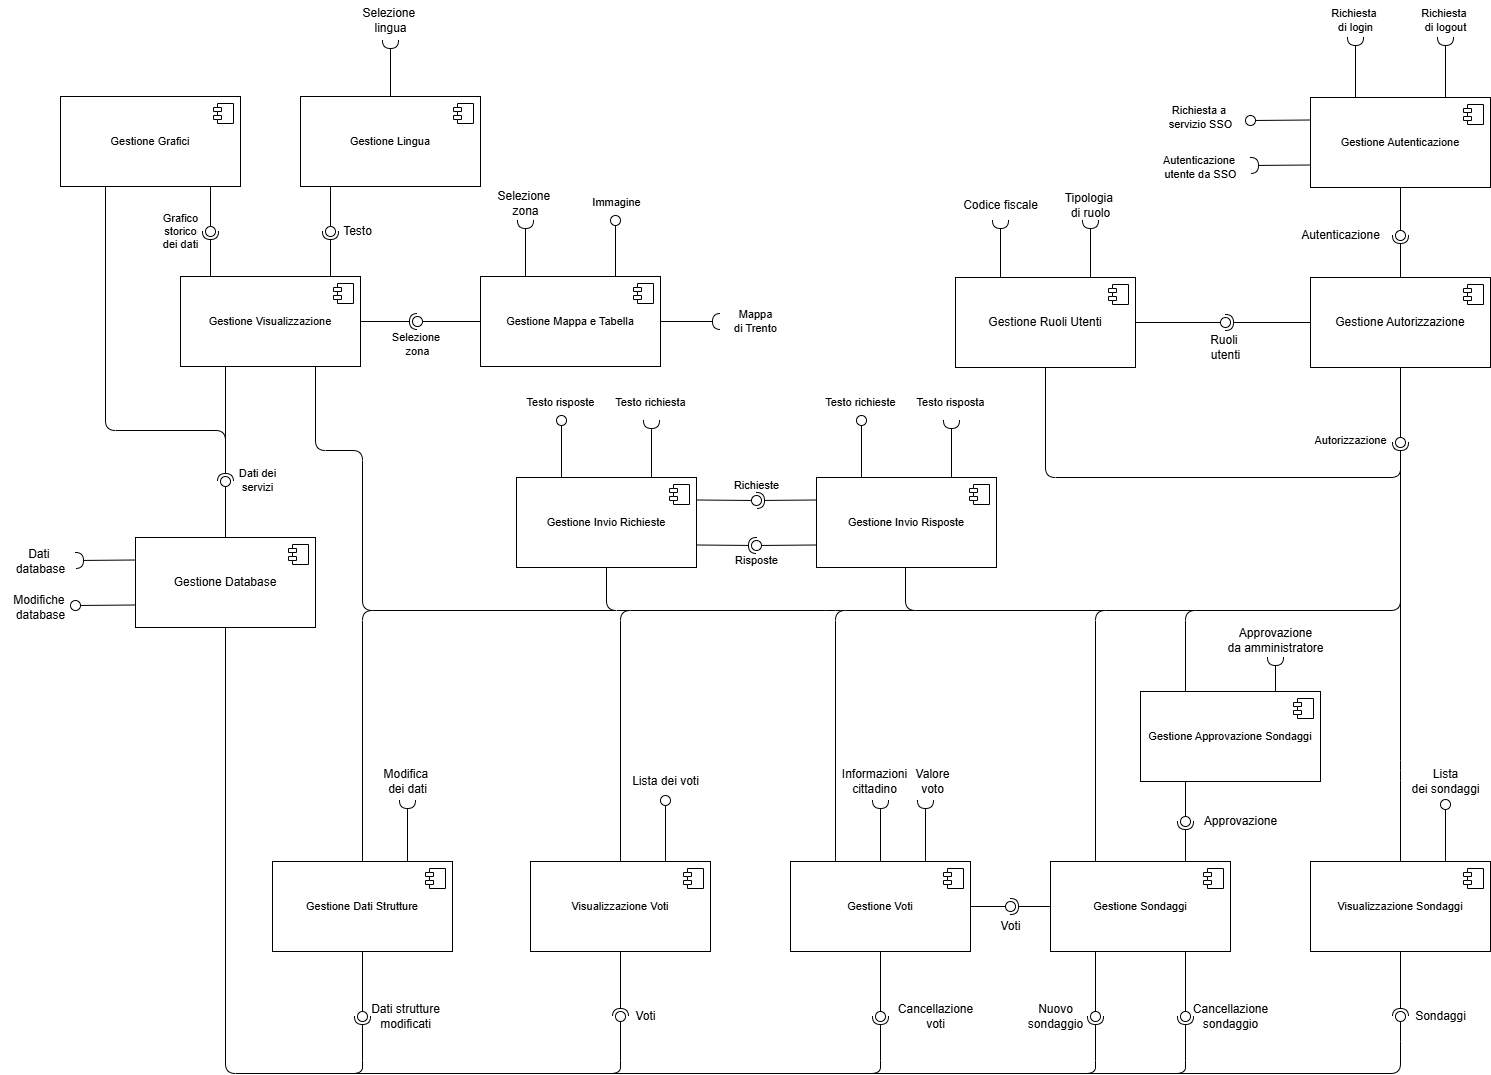
\includegraphics[width=1\textwidth]{ComponentDiagrams/ComponentDiagram.drawio.png}
    \end{figure}